% !TeX root = ../../Book1.tex
% 纲要标题：### 5.4 万有覆盖与分类定理
% 纲要位置：几何学计划纲要.md，第 298 行。
% 正文状态：初稿；尚未正式审核。

% 纲要内容开始
% 
% * 道路类构造和拓扑的定义
% * 局部假设保证覆盖性质
% * 带基点连通覆盖与子群的对应
% * 不带基点的共轭类及正规覆盖
% * 局部假设失败时分类论证在哪里中断
% 
% 纲要内容结束

\section{万有覆盖与分类定理}
\label{g1:sec:0504}

沿圆周行走时，只记录终点会丢掉已经绕过的圈数；把道路提到实线上，这段历史便保留在终点的整数偏移中。一般空间也可以尝试保留从某个固定点出发的全部道路历史。不过，连续变形不应产生新的历史，所以真正要记录的是定端点同伦类。这样得到的集合是否仍能在每一点附近看起来像原空间，正是本节首先要解决的问题。解决以后，覆盖的不同之处就可以解释为：允许把哪些环路的历史遗忘掉。

\subsection{道路类构造和拓扑的定义}
\label{g1:subsec:0504:01}

局部收缩条件有两种不同的范围。邻域中的环路能够在整个空间中缩掉，并不表示它能够在这个邻域内部缩掉。

\begin{definition}[半局部单连通]\label{g1:def:semilocally-simply-connected}
	设 \(X\) 为拓扑空间。如果每个 \(x\in X\) 都有开邻域 \(U\)，使每条以 \(x\) 为基点、完全位于 \(U\) 的环路在 \(X\) 中定基点零伦，即包含映射诱导的同态 \(\pi_1(U,x)\to\pi_1(X,x)\) 为零，就称该空间为\term[banjubudanliantong]{半局部单连通}[semilocally simply connected]。若每一点都有由单连通开邻域组成的邻域基，则称 \(X\)\term[jubudanliantong]{局部单连通}[locally simply connected]。
\end{definition}

局部单连通蕴含局部道路连通与半局部单连通；本节的分类定理只要求后两项。若 \(X\) 局部道路连通且半局部单连通，则每个开邻域 \(O\ni x\) 都包含一个道路连通开邻域 \(U\ni x\)，使 \(U\) 中的全部环路在 \(X\) 中零伦。事实上，先取半局部条件中的邻域 \(W\)，再在 \(W\cap O\) 内取道路连通开邻域 \(U\)。以 \(x\) 为基点的结论成立；以其他 \(y\in U\) 为基点的环路，可以沿 \(U\) 内一条从 \(x\) 到 \(y\) 的道路搬回 \(x\)，由\cref{g1:prop:basepoint-change}得到同样结论。下文把这样的道路连通开集 \(U\) 简称为好邻域；它不必本身单连通。

固定 \(x_0\in X\)。令 \(\widetilde X\) 为所有从 \(x_0\) 出发的道路的定端点同伦类所成的集合，定义
\[
	\widetilde x_0=[e_{x_0}],\qquad p:\widetilde X\longrightarrow X,\qquad p([\alpha])=\alpha(1).
\]
这里 \(e_{x_0}\) 是常值道路，符号 \([\alpha]\) 包含终点信息：不同终点的道路不可能代表同一个点。如何描述 \([\alpha]\) 附近的点？合理的选择是保留已有道路，只允许在它的末端追加一小段道路。若 \(U\) 是包含 \(\alpha(1)\) 的好邻域，令
\[
	B([\alpha],U)=\{[\alpha*\beta]:\beta(0)=\alpha(1),\ \beta(I)\subseteq U\}.
\]
沿用全章约定，\(\alpha*\beta\) 表示先走 \(\alpha\)，再走 \(\beta\)。改变 \(\alpha\) 的同伦代表不改变上述集合，因为道路拼接与定端点同伦相容，见\cref{g1:prop:path-classes}。

\begin{lemma}[道路类的基本邻域]\label{g1:lem:path-class-basis}
	设 \(X\) 道路连通、局部道路连通且半局部单连通，固定 \(x_0\in X\)。令 \(\widetilde X\) 为从 \(x_0\) 出发的道路的定端点同伦类集合，\(p([\alpha])=\alpha(1)\)。对含 \(\alpha(1)\) 的道路连通开集 \(U\)，要求其中所有基于 \(\alpha(1)\) 的环路在 \(X\) 中零伦，并记 \(B([\alpha],U)=\{[\alpha*\beta]:\beta:[0,1]\to U,\ \beta(0)=\alpha(1)\}\)。所有 \(B([\alpha],U)\) 构成 \(\widetilde X\) 的一个拓扑基；在此拓扑下，限制映射 \(p:B([\alpha],U)\to U\) 是同胚。
\end{lemma}
\begin{proof}
	每个 \([\alpha]\) 都属于这样的集合，因为可以追加常值道路。若 \([\delta]\in B([\alpha],U)\cap B([\gamma],V)\)，取包含 \(\delta(1)\) 的好邻域 \(W\subseteq U\cap V\)。由 \([\delta]=[\alpha*\beta]\)、\(\beta(I)\subseteq U\)，在 \(\delta\) 后追加一条位于 \(W\) 的道路，仍然得到 \(B([\alpha],U)\) 中的点；对 \(V\) 同理。所以
	\[
		B([\delta],W)\subseteq B([\alpha],U)\cap B([\gamma],V),
	\]
	这就验证了拓扑基的交集条件。

	限制映射满射，因为 \(U\) 道路连通。若 \(\beta,\beta'\) 从 \(\alpha(1)\) 出发并在 \(U\) 内到达同一个点，则 \(\beta*\bar\beta'\) 是 \(U\) 中的环路，在 \(X\) 中零伦。因此 \(\alpha*\beta\) 与 \(\alpha*\beta'\) 定端点同伦，限制映射也单射。这是好邻域条件的第一次关键使用：追加道路的终点已经决定了追加后的历史。

	对 \(X\) 中开集 \(O\) 及任意 \([\delta]\in p^{-1}(O)\)，在 \(O\) 内取 \(\delta(1)\) 的好邻域 \(W\)，则 \(B([\delta],W)\subseteq p^{-1}(O)\)。故 \(p\) 连续。另一方面，\(p\) 将每个基元素 \(B([\delta],W)\) 映为开集 \(W\)，因而是开映射。限制到一个开基元素后，仍是开映射；所以刚才得到的连续双射 \(B([\alpha],U)\to U\) 是同胚。
\end{proof}

这个拓扑记录道路的同伦历史：一个基本邻域保留已有道路，允许在末端追加位于 \(U\) 内的一小段道路。

\subsection{局部假设保证覆盖性质}
\label{g1:subsec:0504:02}

终点映射在每个基本邻域上已经是同胚。要使它成为单连通覆盖，还要证明同一底邻域上方互不相同的基本邻域彼此不交，并把总空间的环路转回道路类来计算。

\begin{definition}[万有覆盖]\label{g1:def:universal-cover}
	覆盖映射 \(p:\widetilde X\to X\) 的总空间若单连通，即非空、道路连通且基本群平凡，则称它为 \(X\) 的\term[wanyoufugai]{万有覆盖}[universal covering]。
\end{definition}

\begin{theorem}[道路类构造万有覆盖]\label{g1:thm:path-class-universal-cover}
	设 \(X\) 道路连通、局部道路连通且半局部单连通，\(x_0\in X\)。令 \(\widetilde X\) 为从 \(x_0\) 出发的道路的定端点同伦类集合。称道路连通开集 \(U\) 为好邻域，是指其中的环路在 \(X\) 中均为零伦；以 \(B([\alpha],U)=\{[\alpha*\beta]:\beta:[0,1]\to U,\ \beta(0)=\alpha(1)\}\) 为基赋予 \(\widetilde X\) 拓扑，其中 \(U\) 遍历含 \(\alpha(1)\) 的好邻域。记 \(\widetilde x_0=[e_{x_0}]\)、\(p([\alpha])=\alpha(1)\)。则 \(p:(\widetilde X,\widetilde x_0)\to(X,x_0)\) 是万有覆盖，每个好邻域都被 \(p\) 均匀覆盖。
\end{theorem}
\begin{proof}
	先固定好邻域 \(U\) 及 \(u\in U\)。在 \(p^{-1}(u)\) 中的每个道路类 \([\alpha]\) 上取基本邻域 \(B([\alpha],U)\)。这些集合覆盖 \(p^{-1}(U)\)：若 \([\eta]\) 的终点是 \(z\in U\)，取 \(U\) 内从 \(u\) 到 \(z\) 的道路 \(\beta\)，则 \([\eta*\bar\beta]\in p^{-1}(u)\)，且 \([\eta]\in B([\eta*\bar\beta],U)\)。

	不同的 \([\alpha],[\alpha']\in p^{-1}(u)\) 给出互不相交的基本邻域。否则可写 \([\alpha*\beta]=[\alpha'*\beta']\)，其中 \(\beta,\beta'\) 在 \(U\) 内由 \(u\) 到达同一点。环路 \(\beta*\bar\beta'\) 在 \(X\) 中零伦，故消去末端道路后得到 \([\alpha]=[\alpha']\)。结合\cref{g1:lem:path-class-basis}中的局部同胚，得到
	\[
		p^{-1}(U)=\coprod_{[\alpha]\in p^{-1}(u)}B([\alpha],U).
	\]
	道路连通性还保证 \(p\) 满射，所以这确实是覆盖映射。

	下面证明总空间道路连通。对任意道路 \(\alpha\) 定义初段 \(\alpha_t(s)=\alpha(ts)\)，则
	\[
		\widetilde\alpha(t)=[\alpha_t],\qquad 0\le t\le1
	\]
	从 \(\widetilde x_0\) 走到 \([\alpha]\)。它连续：在任意 \(t_0\) 附近，取好邻域 \(U\ni\alpha(t_0)\)，再把参数区间缩小，使相应的道路小段都在 \(U\) 内。无论 \(t\ge t_0\) 还是 \(t\le t_0\)，\([\alpha_t]\) 都可由 \([\alpha_{t_0}]\) 追加这段道路或其反路得到。因此在此区间内 \(\widetilde\alpha\) 等于局部逆 \((p|_{B([\alpha_{t_0}],U)})^{-1}\circ\alpha\)，从而连续。

	最后设 \(\lambda\) 是 \(\widetilde X\) 中以 \(\widetilde x_0\) 为基点的环路，令 \(\alpha=p\circ\lambda\)。上面的初段构造给出 \(\alpha\) 从 \(\widetilde x_0\) 出发的提升；由\cref{g1:thm:path-lifting}的唯一性，它就是 \(\lambda\)。因此 \([\alpha]=\widetilde\alpha(1)=\widetilde x_0\)，即 \(\alpha\) 在 \(X\) 中零伦。由\cref{g1:prop:covering-pi1-injective}，覆盖诱导的 \(p_*\) 是单射，所以 \([\lambda]=1\)。这证明了 \(\widetilde X\) 单连通。
\end{proof}

这个证明显示了两个局部条件的不同职责。局部道路连通使好邻域足够多，能够恢复 \(X\) 的原拓扑；半局部单连通则使每片基本邻域不会因绕小圈而在同一个终点上产生多个历史。

\begin{corollary}[万有覆盖向任意连通覆盖的映射]\label{g1:cor:universal-cover-map}
	设 \(X\) 为局部道路连通拓扑空间，\(x_0\in X\)，\(p:(\widetilde X,\widetilde x_0)\to(X,x_0)\) 是万有覆盖（其道路类构造见\cref{g1:thm:path-class-universal-cover}），\(q:(E,e_0)\to(X,x_0)\) 是连通覆盖。存在唯一连续映射 \(F:\widetilde X\to E\)，使 \(qF=p\)、\(F(\widetilde x_0)=e_0\)；这个 \(F\) 本身也是满射覆盖映射。
	\[
		\begin{tikzcd}
			(\widetilde X,\widetilde x_0)\arrow[rr,dashed,"F"]\arrow[dr,"p"']&&(E,e_0)\arrow[dl,"q"]\\
			&(X,x_0)&
		\end{tikzcd}
	\]
\end{corollary}
\begin{proof}
	覆盖的局部同胚性质使 \(E\) 与 \(\widetilde X\) 局部道路连通；因此连通的 \(E\) 道路连通，见\cref{g1:thm:locally-path-components}。因为 \(\pi_1(\widetilde X)=1\)，\cref{g1:thm:lifting-criterion}的子群包含条件自动满足，给出所需唯一映射。任取 \(e\in E\)，沿 \(E\) 中从 \(e_0\) 到 \(e\) 的道路投影，再提升到 \(\widetilde X\)。由提升唯一性，所得末端映到 \(e\)，所以 \(F\) 满射。

	在 \(X\) 中取一个道路连通开邻域 \(U\)，使它同时被 \(p,q\) 均匀覆盖。\(p\) 的每一片道路连通，故其在 \(F\) 下的像落在 \(q\) 的一片中，且在这两片上 \(F=(q|_{\text{该片}})^{-1}\circ p\)，是同胚。对 \(q\) 的任一片，其逆像便是若干这样的 \(p\) 的片的不交并。这说明 \(F\) 是覆盖映射。
\end{proof}

\subsection{带基点连通覆盖与子群的对应}
\label{g1:subsec:0504:03}

令 \(G=\pi_1(X,x_0)\)。前节已经说明，一个带基点覆盖 \(q:(E,e_0)\to(X,x_0)\) 决定子群 \(q_*\pi_1(E,e_0)\le G\)：它恰好收集那些从 \(e_0\) 出发后仍回到 \(e_0\) 的环路类。现在反过来，从指定子群 \(H\le G\) 出发构造覆盖。两条道路 \(\alpha,\beta\) 应被认为具有相同历史，当且仅当它们终点相同，而且相差的环路 \(\alpha*\bar\beta\) 属于 \(H\)。也就是说，\(H\) 指定了允许遗忘的环路。

\begin{theorem}[子群对应的覆盖]\label{g1:thm:subgroup-covering}
	设 \(X\) 道路连通、局部道路连通且半局部单连通，\(x_0\in X\)，\(H\le G=\pi_1(X,x_0)\)。在从 \(x_0\) 出发的道路集合上规定
	\[
		\alpha\sim_H\beta\quad\Longleftrightarrow\quad
		\alpha(1)=\beta(1)\ \text{且}\ [\alpha*\bar\beta]\in H.
	\]
	以 \([\alpha]_H\) 记等价类，令 \(E_H\) 为这些等价类的集合，\(e_H=[e_{x_0}]_H\)。以
	\[
		B_H([\alpha]_H,U)=\{[\alpha*\beta]_H:\beta:[0,1]\to U,\ \beta(0)=\alpha(1)\}
	\]
	为基赋予拓扑，其中 \(U\) 遍历含 \(\alpha(1)\) 的道路连通开邻域，且 \(U\) 中所有基于 \(\alpha(1)\) 的环路均在 \(X\) 中零伦。则终点映射 \(p_H:(E_H,e_H)\to(X,x_0)\) 是连通覆盖，且
	\[
		(p_H)_*\pi_1(E_H,e_H)=H,\qquad p_H^{-1}(x_0)\cong H\backslash G=\{Hg:g\in G\}.
	\]
	尤其覆盖的叶数为子群指数 \([G:H]\)，允许此数无限。
\end{theorem}
\begin{proof}
	关系自反、对称分别来自单位元与取逆。若 \(\alpha\sim_H\beta\)、\(\beta\sim_H\gamma\)，则
	\[
		[\alpha*\bar\gamma]=[\alpha*\bar\beta]\,[\beta*\bar\gamma]\in H,
	\]
	其中消去 \(\bar\beta*\beta\) 用的是道路类的拼接与逆关系。因此这是等价关系；特别地，同伦的道路必等价。若 \([\alpha]_H=[\alpha']_H\)，追加同一条 \(\beta\) 不改变等价性，因为 \([\alpha*\beta*\bar\beta*\bar\alpha']=[\alpha*\bar\alpha']\)。于是基元素的定义不依赖代表。

	基的交集条件与\cref{g1:lem:path-class-basis}相同：若 \([\delta]_H\) 在两个基元素中，在两好邻域交内取更小好邻域 \(W\)，则 \(B_H([\delta]_H,W)\) 同时包含在二者之内。每个 \(B_H([\alpha]_H,U)\to U\) 满射。若两个追加道路终点相同，它们在 \(U\) 中相差的环路在 \(X\) 中为单位元，因而属于 \(H\)，故此限制映射单射。它的连续性与开性也由同一基论证得到，所以是同胚。

	固定 \(u\in U\)，这些基元素在 \([\alpha]_H\) 遍历 \(p_H^{-1}(u)\) 时覆盖 \(p_H^{-1}(U)\)。若其中两片相交，则有 \([\alpha*\beta]_H=[\alpha'*\beta']_H\)，其中 \(\beta,\beta'\) 都在 \(U\) 内由 \(u\) 到达同一点。由于 \(\beta*\bar\beta'\) 在 \(X\) 中零伦，等价条件化为 \([\alpha*\bar\alpha']\in H\)，即两个索引本来就相同。因此这些片互不相交，\(p_H\) 是覆盖。初段道路 \(t\mapsto[\alpha_t]_H\) 的连续性由局部逆证明，故 \(E_H\) 道路连通。

	以 \(x_0\) 为基点的环路 \(\gamma\) 从 \(e_H\) 出发提升后终点为 \([\gamma]_H\)，它等于 \(e_H\) 当且仅当 \([\gamma]\in H\)。\cref{g1:cor:closed-lift-criterion}告诉我们，闭提升的环路类恰为 \((p_H)_*\pi_1(E_H,e_H)\)，所以该子群正是 \(H\)。纤维内的道路全是环路；若其类为 \(g,k\in G\)，等价条件为 \(gk^{-1}\in H\)，等价于 \(Hg=Hk\)。这给出所述纤维对应。其他纤维与此纤维之间可沿一条道路提升得到双射，故叶数恒为 \([G:H]\)。
\end{proof}

\begin{theorem}[带基点的连通覆盖分类]\label{g1:thm:based-covering-classification}
	设 \(X\) 道路连通、局部道路连通且半局部单连通，\(x_0\in X\)。带基点连通覆盖 \(q:(E,e_0)\to(X,x_0)\) 的等价类与 \(G=\pi_1(X,x_0)\) 的子群一一对应；这里等价指保持基点且与投影交换的同胚。对应把 \((E,e_0)\) 送到 \(q_*\pi_1(E,e_0)\)，逆对应把子群 \(H\le G\) 送到满足 \(q_*\pi_1(E,e_0)=H\) 的唯一带基点连通覆盖等价类。
\end{theorem}
\begin{proof}
	给定覆盖，令 \(H=q_*\pi_1(E,e_0)\)。总空间 \(E\) 局部道路连通，且连通，因而道路连通。定义 \(F:E_H\to E\)：把 \([\alpha]_H\) 送到 \(\alpha\) 从 \(e_0\) 出发的提升终点。需要证明，此终点恰好只忘掉 \(H\) 中的历史。

	若 \(\alpha,\beta\) 有相同终点，则其提升终点相同，当且仅当 \(\alpha*\bar\beta\) 有从 \(e_0\) 出发的闭提升。一方向可以直接把两条提升拼接；反方向把闭提升分为前后两段，反转后半段，再用 \(\beta\) 的提升唯一性。由闭提升判据，这又等价于 \([\alpha*\bar\beta]\in H\)。所以 \(F\) 良定义且单射。任意 \(e\in E\) 可沿 \(E\) 中一条从 \(e_0\) 到 \(e\) 的道路到达，取其投影就得 \(F\) 的一个原像，因此 \(F\) 满射。

	对 \([\alpha]_H\)，取包含 \(\alpha(1)\) 的好邻域 \(U\)，并使它被 \(q\) 均匀覆盖。在 \(B_H([\alpha]_H,U)\) 上，\(F\) 就是 \(p_H\) 后接经过 \(F([\alpha]_H)\) 的那片的局部逆。因此 \(F\) 局部为同胚，进而是同胚，且 \(qF=p_H\)、\(F(e_H)=e_0\)。

	如果两个带基点覆盖等价，等价同胚诱导基本群同构，故它们在 \(G\) 中的像子群相同；反过来，若像子群相同，上述构造说明它们都与同一个 \(E_H\) 等价。最后，\cref{g1:thm:subgroup-covering}保证每个子群确实出现，完成一一对应的证明。
\end{proof}

\(H=\{1\}\) 时，上述构造就是万有覆盖；\(H=G\) 时，所有同终点道路都等价，得到恒等覆盖 \(X\to X\)。子群越大，允许遗忘的历史越多，覆盖中的点就越少。万有覆盖的“万有”对应\cref{g1:cor:universal-cover-map}所述的映射性质。

\subsection{不带基点的共轭类及正规覆盖}
\label{g1:subsec:0504:04}

同一个覆盖若换了纤维中的起点，能够闭合的环路集合也可能改变。为看清改变方式，暂将从 \(e\in q^{-1}(x_0)\) 提升代表 \(g\in G\) 的环路所得终点记为 \(e\cdot g\)。同伦提升保证它与代表无关，先走后走的约定给出
\[
	(e\cdot g)\cdot k=e\cdot(gk),\qquad e\cdot1=e.
\]
这就是纤维上的右作用。连通覆盖的总空间道路连通，所以此作用传递：任意两个纤维点可由道路相连，其投影是所需环路。对 \(E_H\)，纤维对应 \(H\backslash G\)，且右作用为 \((Hg)\cdot k=H(gk)\)。于是
\[
	\{k:(Hg)\cdot k=Hg\}=g^{-1}Hg.
\]
左边是以 \(Hg\) 为起点时有闭提升的环路类，因而也是该基点处基本群在 \(G\) 中的像。

\begin{proposition}[不带基点的分类]\label{g1:prop:unbased-covering-classification}
	设 \(X\) 道路连通、局部道路连通且半局部单连通，\(x_0\in X\)。不指定总空间基点的连通覆盖等价类，与 \(\pi_1(X,x_0)\) 的子群共轭类一一对应。
\end{proposition}
\begin{proof}
	在同一个连通覆盖内换基点，刚才的计算说明像子群由 \(H\) 变成 \(g^{-1}Hg\)，且所有这样的共轭子群都可得到。若两个不带基点的覆盖等价，任选第一个覆盖的一个纤维点，并在第二个中选它的像，便得到相同的像子群；与第二个覆盖原来任选的基点比较，只相差共轭。反过来，若两个覆盖的像子群共轭，可以在其中一个覆盖内更换纤维基点，使两个像子群相同，再应用\cref{g1:thm:based-covering-classification}得到等价。
\end{proof}

\begin{definition}[正规覆盖]\label{g1:def:normal-covering}
	连通覆盖 \(q:E\to X\) 若其覆盖变换群在每个纤维上传递，称为\term[zhengguifugai]{正规覆盖}[regular covering]；英文文献也使用 normal covering。\foreignidx{normal covering}在道路连通底空间上，只需在一个纤维上传递：沿连接两个底点的道路提升，可把覆盖变换与两纤维间的对应交换。
\end{definition}

正规性允许在覆盖内部把任一张“同样的片”搬到另一张。这个要求比“各纤维点数相同”强得多，后者对这里所有覆盖都成立。

\begin{theorem}[正规化子与覆盖变换]\label{g1:thm:normal-covering-deck}
	设 \(X\) 道路连通、局部道路连通且半局部单连通，\(x_0\in X\)，\(G=\pi_1(X,x_0)\)，\(H\le G\)。令 \(p_H:(E_H,e_H)\to(X,x_0)\) 为满足 \((p_H)_*\pi_1(E_H,e_H)=H\) 的带基点连通覆盖。记
	\[
		N_G(H)=\{n\in G:nHn^{-1}=H\}.
	\]
	这个子群称为 \(H\) 在 \(G\) 中的\term[zhengguihuazi]{正规化子}[normalizer]。则有群同构
	\[
		\operatorname{Deck}(E_H/X)\cong N_G(H)/H.
	\]
	覆盖 \(E_H\to X\) 正规当且仅当 \(H\) 是 \(G\) 的正规子群；此时覆盖变换群为 \(G/H\)。特别地，万有覆盖的覆盖变换群同构于 \(G\)，在道路类模型上由
	\[
		L_g[\alpha]=[\gamma*\alpha],\qquad [\gamma]=g
	\]
	给出左作用，并且 \(L_g\circ L_k=L_{gk}\)。
\end{theorem}
\begin{proof}
	先构造变换，再说明没有遗漏。若 \(n\in N_G(H)\)，选代表环路 \(\nu\)，令 \(L_n[\alpha]_H=[\nu*\alpha]_H\)。若 \([\alpha]_H=[\beta]_H\)，则
	\[
		[\nu*\alpha*\bar\beta*\bar\nu]
		=n[\alpha*\bar\beta]n^{-1}\in H,
	\]
	所以公式良定义，也不依赖 \(\nu\) 的同伦代表。它把 \(B_H([\alpha]_H,U)\) 同胚地送到 \(B_H([\nu*\alpha]_H,U)\)，逆为 \(L_{n^{-1}}\)，并保持投影，故是覆盖变换。拼接顺序直接给出 \(L_m\circ L_n=L_{mn}\)，这是到覆盖变换群的同态。\(L_n\) 为恒等当且仅当 \(n\in H\)：一方向代入基点 \(e_H\)；另一方向用 \([\nu*\alpha*\bar\alpha]=n\in H\)。因此核为 \(H\)。

	任一覆盖变换 \(T\) 都与纤维的右作用交换，因为 \(T\) 将一条道路的提升变成从像点出发的同一道路的提升，而提升唯一。写 \(T(e_H)=Hn\)。由 \(T\) 可逆，一个 \(g\) 固定 \(e_H\) 当且仅当它固定 \(T(e_H)\)。前者的稳定子是 \(H\)，后者是 \(n^{-1}Hn\)，所以 \(n^{-1}Hn=H\)，即 \(n\in N_G(H)\)。\(T\) 与 \(L_n\) 在 \(e_H\) 相等，由\cref{g1:prop:deck-determined}，它们在整个连通覆盖上相等。故上述同态满射，商去核得到群同构。

	基点 \(e_H\) 的覆盖变换轨道恰为 \(\{Hn:n\in N_G(H)\}\)。它等于全部纤维 \(H\backslash G\)，当且仅当 \(N_G(H)=G\)：若 \(Hg=Hn\)，则 \(g\in Hn\subseteq N_G(H)\)。而 \(N_G(H)=G\) 正是 \(H\trianglelefteq G\)。正规性与正规子群条件的等价因而成立。最后令 \(H=\{1\}\)，就得到万有覆盖的结论。
\end{proof}

这里的左右两种作用承担不同任务。覆盖变换群在道路前面追加环路，所以是左作用；纤维的路径提升在道路后面追加环路，所以是右作用。在 \(H\backslash G\) 上，前者写为 \(Hg\mapsto Hng\)（\(n\in N_G(H)\)），后者写为 \(Hg\mapsto Hgk\)（\(k\in G\)）。左右乘相互交换，因而这两类纤维置换彼此相容。

也可以把 \(E_H\) 写成 \(H\backslash\widetilde X\)。事实上，\([\alpha]_H=[\beta]_H\) 等价于存在 \(h\in H\) 使 \([\alpha]=L_h[\beta]\)：取 \(h=[\alpha*\bar\beta]\) 即可。因此自然满射 \(\widetilde X\to E_H\) 的纤维正是 \(H\) 的左轨道。它把基本邻域 \(B([\alpha],U)\) 映为 \(B_H([\alpha]_H,U)\)，是连续开满射，故 \(E_H\) 的拓扑正是此轨道商拓扑。这些基本邻域就是\cref{g1:thm:subgroup-covering}中构造出的覆盖片。

\subsection{局部假设失败时分类论证在哪里中断}
\label{g1:subsec:0504:05}

下面先看半局部单连通失败的空间：它仍然道路连通、局部道路连通，但根本没有单连通覆盖。

\begin{example}[缩小圆周汇聚在同一点]\label{g1:exm:hawaiian-earring}
	在平面中令
	\[
		C_n=\{(x,y):(x-1/n)^2+y^2=1/n^2\},\qquad
		Z=\bigcup_{n\ge1}C_n,\qquad o=(0,0).
	\]
	赋予 \(Z\) 平面的子空间拓扑。这个空间称为\term[xiaweiyierhuan]{Hawaii 耳环}[Hawaiian earring]。所有圆周相交于 \(o\)，所以 \(Z\) 道路连通。非 \(o\) 点附近有普通开弧邻域；\(o\) 附近的 \(Z\cap B(o,\varepsilon)\) 在每个圆周上截得包含 \(o\) 的一段弧或整个圆周，这些集合都能沿弧连到 \(o\)，所以也道路连通。故 \(Z\) 局部道路连通。
	\begin{figure}[htbp]
		\centering
		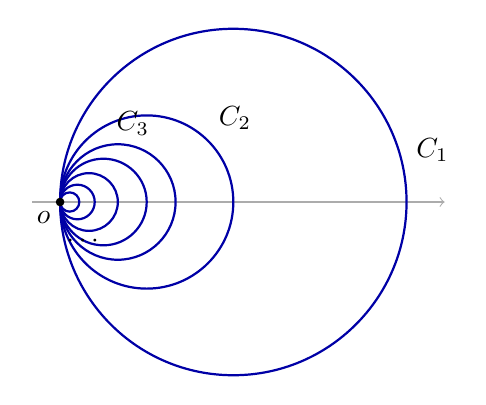
\begin{tikzpicture}[x=2.2cm,y=2.2cm]
	\draw[->,gray!65] (-0.16,0)--(2.22,0);
	\foreach \n in {1,2,3,4,6,10,18}{
		\pgfmathsetmacro{\rad}{1/\n}
		\draw[blue!65!black,thick] (\rad,0) circle[radius=\rad];
	}
	\fill (0,0) circle[radius=0.025];
	\node[below left] at (0,0) {\(o\)};
	\node[right] at (2,0.30) {\(C_1\)};
	\node[above right] at (0.86,0.36) {\(C_2\)};
	\node[above] at (0.42,0.33) {\(C_3\)};
	\node at (0.13,-0.23) {\(\cdots\)};
\end{tikzpicture}
% !TeX root = ../Book1.tex

		\caption{Hawaii 耳环中的若干圆周。图中只画出有限多个；完整空间含全部 \(C_n\)，它们都通过 \(o\)，且直径趋于零。任意小的 \(o\) 的邻域仍包含完整的小圆周。}
		\label{g1:fig:hawaiian-earring}
	\end{figure}

	固定 \(n\)，定义 \(r_n:Z\to C_n\)，在 \(C_n\) 上恒等，在其他圆周上恒取 \(o\)。它连续：在 \(o\) 处有 \(\|r_n(z)\|\le\|z\|\)；在非 \(o\) 点附近，可以避开所有其他圆周，或避开 \(C_n\)，因为足够小的圆周全都挤在 \(o\) 附近，而其余只有有限个。因而 \(r_n\) 是连续缩回。绕 \(C_n\) 一周的环路若在 \(Z\) 中零伦，复合 \(r_n\) 就会使它在 \(C_n\) 中零伦，这与\cref{g1:thm:circle-fundamental}矛盾。

	然而 \(o\) 的每个邻域都包含充分大的 \(n\) 对应的整个 \(C_n\)，因为 \(C_n\subseteq\overline B(o,2/n)\)。所以任意小邻域都有在 \(Z\) 中不能缩掉的环路，\(Z\) 不半局部单连通。

	若存在单连通覆盖 \(q:Y\to Z\)，取 \(o\) 的均匀覆盖邻域 \(U\) 及其上面任意一片。充分小的整个 \(C_n\) 位于 \(U\)；绕它一周的环路可经该片的局部逆提升为 \(Y\) 中的环路。它在单连通的 \(Y\) 中零伦，投影后便在 \(Z\) 中零伦，矛盾。因此 \(Z\) 不存在万有覆盖。这个论证只使用单个圆周的基本群，不需要描述 \(\pi_1(Z,o)\) 的全部结构。
\end{example}

在道路类构造中，失败发生在一个明确位置：如果邻域 \(U\) 中还有在 \(X\) 内非零伦的环路 \(\beta\)，则 \([\alpha]\) 与 \([\alpha*\beta]\) 有相同投影，却未必相同。因此 \(B([\alpha],U)\to U\) 可能不单射，也就不能作为覆盖的一片。

局部道路连通的职责则不同。\cref{g1:exm:topologist-sine}中的拓扑正弦曲线 \(S\) 在竖直线段上的道路分支不是开集，故没有道路连通开邻域基。取它的锥，可以保留局部道路连通性的障碍，同时使整个空间可缩：
\[
	C(S)=\{((1-t)x,(1-t)y,t):(x,y)\in S,\ 0\le t\le1\}\subseteq\mathbb R^3.
\]
顶点为 \(v=(0,0,1)\)。每个点都能沿直线连到 \(v\)，且直线同伦 \((z,s)\mapsto(1-s)z+sv\) 始终留在锥中，因此 \(C(S)\) 可缩，特别是道路连通、单连通并半局部单连通。不过在开集 \(V=\{t<1/2\}\cap C(S)\) 内，坐标变换
\[
	((1-t)x,(1-t)y,t)\longmapsto((x,y),t)
\]
给出 \(V\cong S\times[0,1/2)\)。点 \(((0,0),0)\) 的每个相对开邻域都遇到正弦图像上的点；若它有包含于 \(V\) 的道路连通开邻域，投影到 \(S\) 就会给出从竖直线段到正弦图像的道路，与\cref{g1:exm:topologist-sine}矛盾。因此这个单连通空间仍不局部道路连通。在它上面，恒等映射当然是万有覆盖，但上述“在任意给定邻域内取好邻域”的拓扑基论证不能照搬。

在道路类构造中，半局部单连通保证局部单射，局部道路连通保证好邻域构成原拓扑的基。锥的例子同时说明，特定空间即使缺少后一个条件，也可能有万有覆盖。关于本节道路类模型与覆盖分类的进一步阅读，可参见\cite[第1.3节]{Hatcher2002}。
